\documentclass[letterpaper]{article}

\usepackage{fancyvrb}
\usepackage{fullpage}
\usepackage{listings}
\usepackage{xcolor}
\usepackage{float}
\usepackage{hyperref}

\lstset{basicstyle=\ttfamily, 
        backgroundcolor=\color[gray]{0.95}}
        
\author{Michael Gruenstaeudl, Nils Jenke}
\title{Using the PACViR Pipeline}

\usepackage{Sweave}
\begin{document}
\Sconcordance{concordance:PACViR_Vignette.tex:PACViR_Vignette.Rnw:%
1 15 1 1 0 3 1 1 4 16 1 5 0 1 4 9 1 1 3 2 0 1 3 1 0 1 %
1 1 2 6 1 4 0 1 3 35 1 1 2 24 0 1 2 1 1}

%\SweaveUTF8


\maketitle

\tableofcontents

\section{Introduction}

  The PACViR pipeline generates a visualization of a plastome in a circular fashion. This vignette provides two examples of   how to execute PACViR via the R function 'PACViR.complete()' and via bash.

\section{Requirements}

  To execute PACViR several requirements have to be installed.


  \begin{footnotesize}
  \begin{lstlisting}[linerange=\\begin\{Sinput\}-\\end\{Sinput\},includerangemarker=false]
\begin{Schunk}
\begin{Sinput}
>     #require(PACViR)
>     require(RCircos)
>     require(genbankr)
>     require(optparse)
\end{Sinput}
\end{Schunk}
  \end{lstlisting}
  \end{footnotesize}


\section{PACViR via R-function }

  PACViR can be easily executed via the PACViR.complete() function in R. Therefore one can load the provided data from the   package.

  \begin{footnotesize}
  \begin{lstlisting}[linerange=\\begin\{Sinput\}-\\end\{Sinput\},includerangemarker=false]
\begin{Schunk}
\begin{Sinput}
>     gbk.file <- "./SCHM2.gb"
>     bam.file <- "./SCHM2.bam"
>     windowSize <- 250
>     mosdepthCmd <- "mosdepth"
>     threshold <- 25 
>     outDir <- "./output"
>     #PACViR.complete(gbk.file, bam.file, windowSize, mosdepthCmd, threshold, outDir)
\end{Sinput}
\end{Schunk}
  \end{lstlisting}
  \end{footnotesize}
  

  \begin{figure}[H]
  \centering
    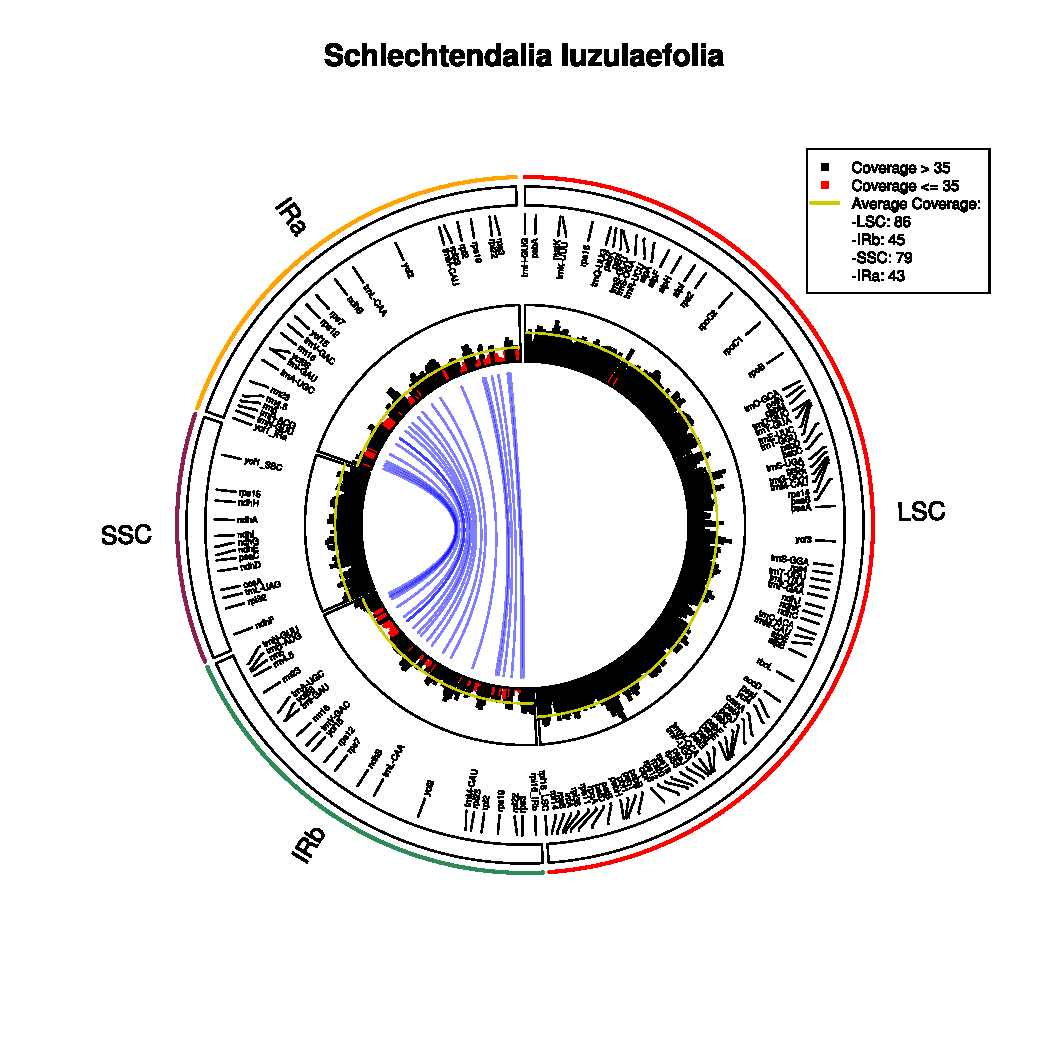
\includegraphics{SCHM2_WS250_TH35.pdf}
    \caption{Visualization of SCHM2 plastome with PACViR.complete()}
  \centering
  \end{figure}

\section{PACViR via command line}

  Execute PACViR\_Rscript.R via command line with Rscript.
  
\begin{footnotesize}
\begin{lstlisting}
  Rscript PACViR_Rscript.R  -k ../inst/extdata/DAS01.gb -b ../inst/extdata/DAS01.bam 
\end{lstlisting}
\end{footnotesize}

  \begin{figure}[H]
  \centering
    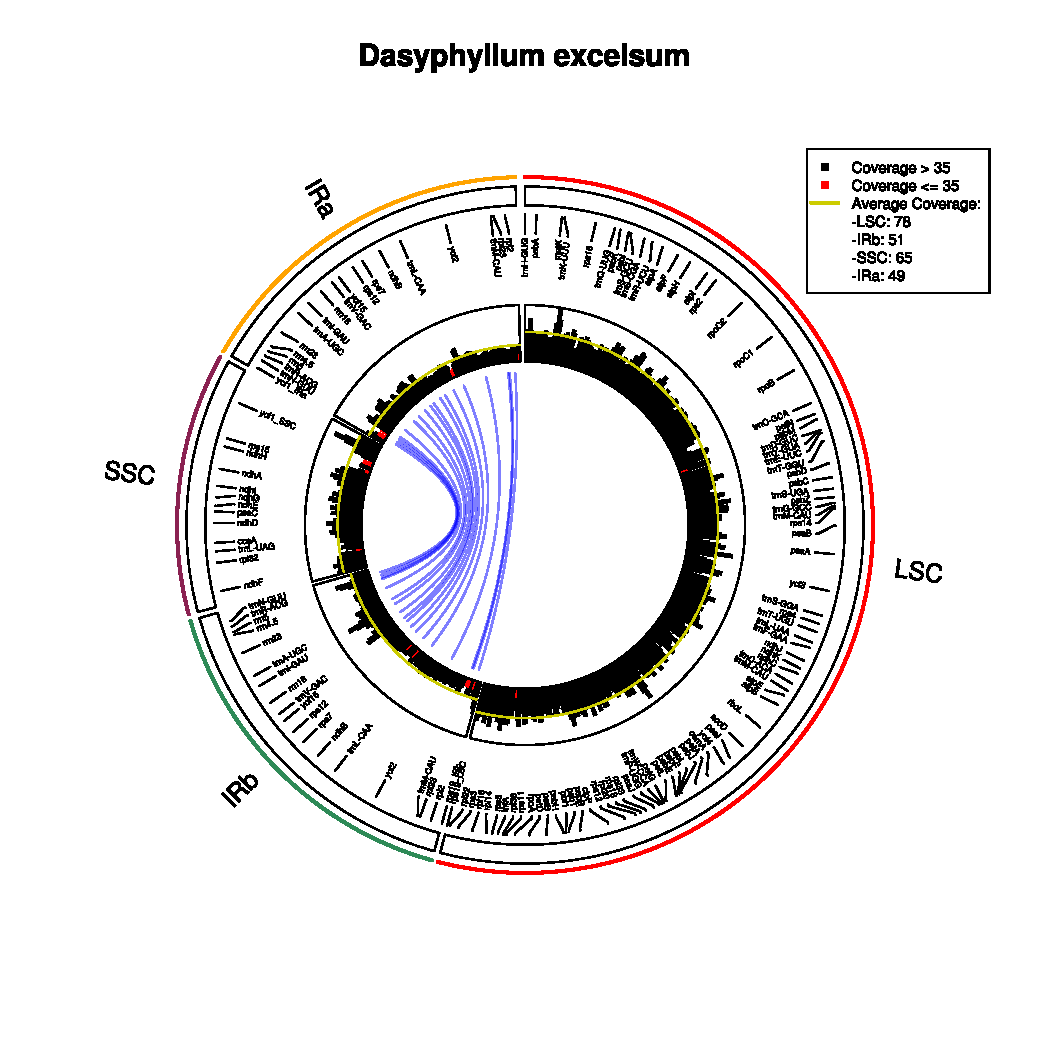
\includegraphics{DAS01_WS250_TH35.pdf}
    \caption{Visualization of DAS01 plastome with Rscript}
  \centering
  \end{figure}
  
\section{Modifying parameters}

  Depending on which system PACViR will be executed

\section{More Information}

\section{sessionInfo}

\begin{Schunk}
\begin{Sinput}
> sessionInfo()
\end{Sinput}
\begin{Soutput}
R version 3.3.3 (2017-03-06)
Platform: x86_64-pc-linux-gnu (64-bit)
Running under: Debian GNU/Linux 9 (stretch)

locale:
[1] C

attached base packages:
[1] stats     graphics  grDevices utils     datasets 
[6] methods   base     

other attached packages:
[1] optparse_1.6.0 genbankr_1.2.1 RCircos_1.2.0 

loaded via a namespace (and not attached):
 [1] Rcpp_1.0.0                 AnnotationDbi_1.36.2      
 [3] XVector_0.14.1             GenomicAlignments_1.10.0  
 [5] GenomicRanges_1.26.4       BiocGenerics_0.20.0       
 [7] zlibbioc_1.20.0            IRanges_2.8.2             
 [9] getopt_1.20.2              BiocParallel_1.8.2        
[11] bit_1.1-14                 BSgenome_1.42.0           
[13] lattice_0.20-35            blob_1.1.1                
[15] GenomeInfoDb_1.10.3        tools_3.3.3               
[17] grid_3.3.3                 SummarizedExperiment_1.4.0
[19] parallel_3.3.3             Biobase_2.34.0            
[21] DBI_1.0.0                  bit64_0.9-7               
[23] digest_0.6.11              Matrix_1.2-7.1            
[25] rtracklayer_1.34.1         S4Vectors_0.12.2          
[27] bitops_1.0-6               RCurl_1.95-4.8            
[29] biomaRt_2.30.0             memoise_1.1.0             
[31] RSQLite_2.1.1              Rsamtools_1.26.2          
[33] GenomicFeatures_1.26.2     Biostrings_2.42.1         
[35] stats4_3.3.3               XML_3.98-1.5              
[37] VariantAnnotation_1.20.2  
\end{Soutput}
\end{Schunk}

\end{document}
